\documentclass[10pt]{beamer}
\usepackage{xeCJK}
\usepackage{listings}
\usepackage{tikz}
\usepackage{subfigure}
\usepackage{color}
\usepackage[ruled,linesnumbered,titlenotnumbered,noend,vlined]{algorithm2e}
\usetikzlibrary{arrows,automata}

\renewcommand{\thealgocf}{}
\newcommand{\sgn}{\textrm{sgn}}

\usetheme[
%	sidebar, % 默认不显示包含幻灯片结构的边框。如设置sidebar选项,则参考AAU模板显示左边框
	footline,
	blue, % 主色调默认为红色,色调可以选择red和blue
%	wide, % 幻灯片的长宽比默认为4:3,如设置了wide选项则为16:9
	hideallsubsections, % 默认显示所有等级的标题。如设置了hideallsubsections,
	                    % 则不显示小节标题
	mathserif, % 默认公式字体是钝化的,如设置mathserif选项则采用正常的公式字体
%	english, % 默认幻灯片环境为中文,如设置english选项则采用英文的章节和图表编号
	sectiontoc, % 设置sectiontoc选项则在每节(section)之前添加一个所有节的目录,
	            % 并标明本节在整个幻灯片中的位置,不建议和\part层级一同使用
]{SEUstyle}

\title[第四组报告]{强化学习与规划 \\ 强化学习在游戏中的应用}
\author[张舒韬 et al.]{刘翔~吴江恒~张舒韬~赵倩隆}
\institute[SEU CS Dept. Team 4]{东南大学\ 计算机科学与工程学院\ 第4组}

\begin{document}
	{\background
		\begin{frame}[plain,noframenumbering]
			\titlepage
		\end{frame}
	}

	\begin{frame}{总目录}
		第I部分 强化学习与规划
		\tableofcontents[part=1]
		第II部分 强化学习在FPS游戏中的应用
		\tableofcontents[part=2]
	\end{frame}

	\part{强化学习与规划}\label{part:rl-and-planning}
	
	\section{背景知识回顾}
	
	\subsection{马尔科夫决策过程}
	
	\begin{frame}{马尔科夫决策过程}{定义}
		\visible<1->{
			一个马尔科夫决策过程是一个五元组$D = \langle S,A,P,r,\gamma \rangle$,其中
			\begin{description}
				\item[$S$] 过程中的状态(state)集合
				\item[$A$] 过程中的动作(action)集合
				\item[$P$] 转移函数(transition function)$P(s, a, s')$定义为$S \times A \times S \rightarrow [0,1]$,表示在状态$s$时选择动作$a$达到状态$s'$的概率
				\item[$r$] 奖励函数(reward function)$r(s, a, s')$定义为$S \times A \times S \rightarrow \mathbb{R}$,表示在状态$s$时选择动作$a$达到状态$s'$时得到的奖励
				\item[$\gamma$] 折扣因子(discount factor)$\gamma \in [0,1]$
			\end{description}
		}
		
		\visible<2->{
			累积奖励的定义
			\begin{equation*}
			\sum^{\infty}_{t=0} {\gamma^t r(s_t, a_t, s_{t+1})}   
			\end{equation*}
		}
	\end{frame}

	\begin{frame}{马尔科夫决策过程}{问题}
		\begin{description}
			\item<2->[预测问题(Predicting)] 已知起始状态、转移函数和决策策略,求在此情况下能够得到的累积奖励的期望;
			\item<3->[规划问题(Planning)] 已知起始状态和转移函数,求使累积奖励的期望值最大的决策策略;
			\item<4->[强化学习(Reinforcement Learning)] 转移函数或奖励函数未知,求使累积奖励的期望值最大的决策策略。
		\end{description}
	\end{frame}

	\begin{frame}{马尔科夫决策过程}{规划与学习}
		\begin{figure}
			\centering
			\begin{tikzpicture}[->,>=stealth',shorten >=1pt,auto,node distance=30cm,semithick,bend angle=40]
			\tikzstyle{every state}=[rectangle,font=\bfseries,fill=white,draw=none,text=black]
			\node (policy) at (0,0)           [state] {value/policy};
			\node (exper)  at (1*2,-1.732*2)  [state] {experience};
			\visible<1,3>{\node (model)  at (-1*2,-1.732*2) [state] {model};}
			
			\path (policy) edge [bend left] node {acting} (exper);
			\visible<1-2>{\path (exper)  edge [bend left] node {direct RL} (policy);}
			\visible<1,3>{\path (exper) edge [bend left] node {model learning} (model);}
			\visible<1,3>{\path (model)  edge [bend left] node {planning} (policy);}
			
			\only<1>{\node at (0,-5.5) [state] { };}
			\only<2>{\node at (0,-5.5) [state,text=red] {Model-Free RL};}
			\only<3>{\node at (0,-5.5) [state,text=red] {Model-Based RL};}
			\end{tikzpicture}
			\caption{学习、规划和执行之间的关系\protect\cite{Sutton1998:RL-Introduction}}\label{fig:relation-in-RL}
		\end{figure}
	\end{frame}

	\subsection{Q-Learning}
	
	\begin{frame}{Q-Learning}{定义}
		\begin{itemize}
			\item<2-> Q-Learning是一种off-policy的时序差分学习方法
			\item<3-> Q-Learning的目标是得到$Q^*$函数的估计,即
			\[Q^*(s,a) = \max_{\pi}\mathbb{E}(R_t | s_t = t, a_t = a, \pi) \]
			\[Q^*(s,a) = \mathbb{E}\left[r_{t+1} + \gamma \max_{a' \in A(s)} Q^*(s_{t+1}, a') | s_t = s, a_t = a\right] \]
			\item<4-> Q-learning的定义为
			\[ Q(s_t, a_t) \gets Q(s_t, a_t) + \alpha \left[r_{t+1} + \gamma \max_{a \in A(s_{t+1})}Q(s_{t+1}, a) - Q(s_t, a_t) \right] \]
		\end{itemize}
	\end{frame}

	\begin{frame}{Q-Learning}{算法描述}
		\begin{algorithm}[H]
			随机初始化$Q(s, a)$\;
			\ForEach{每个周期(episode)}{
				初始化$s$\;
				\ForEach{周期内的每一步,直到$s$为终止状态}{
					利用$Q$函数中获得的策略(例如$\epsilon$-greedy)选择状态$s$时采取的策略\;
					执行$a$,观察$s'$和$r'$\;
					$Q(s_t, a_t) \gets Q(s_t, a_t) + \alpha [r_{t+1} + \gamma \max_{a}Q(s_{t+1}, a) - Q(s_t, a_t) ]$\;
				}
			}
			\caption{Q-Learning}\label{alg:q-learning}
		\end{algorithm}
	\end{frame}

	\begin{frame}{基于强化学习的规划}{Q-Planning}
		
		\begin{figure}
			\centering
			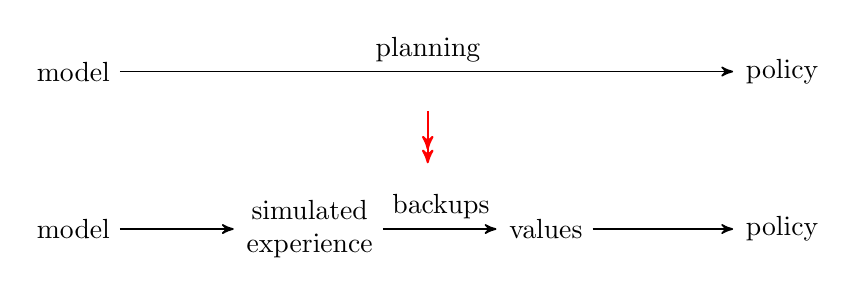
\begin{tikzpicture}[->,>=stealth',shorten >=1pt,auto,node distance=50cm,semithick]
			\tikzstyle{every state}=[rectangle,fill=white,draw=none,text=black,align=center]
				\visible<2->{
					\node (model0) at(0,2) [state] {model};
					\node (policy0) at(9,2) [state] {policy};
					
					\path (model0) edge node {planning} (policy0);
				}
			
				\visible<3-> {
					\draw [->>,thick,draw=red] (4.5,1.5) -- (4.5,0.8);
					\node (model) at(0,0) [state] {model};
					\node (exper) at(3,0) [state] {simulated\\ experience};
					\node (values) at(6,0) [state] {values};
					\node (policy) at(9,0) [state] {policy};
					
					\path (model) edge (exper)
					(exper) edge node {backups} (values)
					(values) edge (policy);
				}
			\end{tikzpicture}
		\end{figure}
	
		\visible<4->{
			\begin{algorithm}[H]
				\Repeat{stop}{
					随机选择$s \in S$, $a \in A(s)$\;
					根据模型模拟出下一状态$s'$和奖励$r$\;
					更新$Q(s,a) \gets Q(s,a) + \alpha[r + \gamma \max_{a'}Q(s',a') - Q(s,a)]$\;
				}
				\caption{随机Q-Planning}
			\end{algorithm}
		}
		
	\end{frame}

	\begin{frame}{强化学习}{强化学习的两种方法}
		\begin{small}		
			\begin{description}
				\item<2->[Model-Based RL] 
				
				优点:
				\begin{itemize}
					\item 有时直接从环境中学到值函数较难,而模型的$P(s’|s,a)$和$R(r|s,a)$很容易就能用监督学习去学;
				\end{itemize}
				
				缺点:
				\begin{itemize}
					\item 误差来源多了模型拟合的误差;
				\end{itemize}
				
				\item<3->[Model-Free RL] 优点:
				\begin{itemize}
					\item 不需要具体的环境模型;
					\item 使用时做出决策的时间快;
				\end{itemize}
				
				缺点:
				\begin{itemize}
					\item 优化过程可能不稳定且不收敛;
					\item 比较难适应变化的环境;
				\end{itemize}
			\end{description}
		\end{small}
	\end{frame}

	\begin{frame}{强化学习}{Model-Free or Model-Based?}
		All models are wrong, but some are useful.
		\begin{flushright}
			--George E.P. Box, Robustness in the strategy of scientific model building
		\end{flushright}
	
		\begin{figure}
			\centering
			\begin{tikzpicture}
				\visible<2->{\node at (0,0) {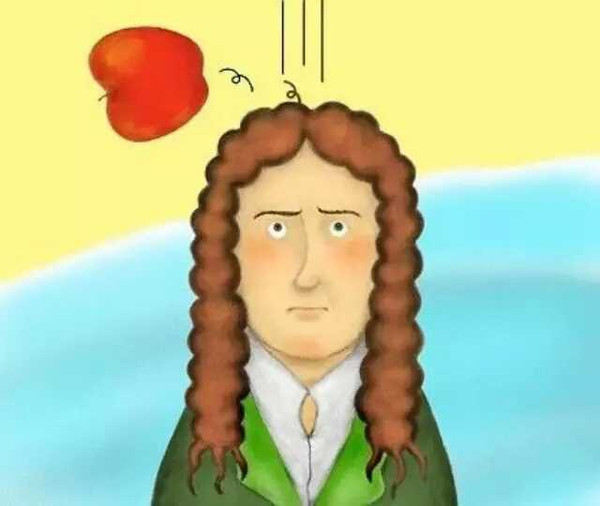
\includegraphics[width=.4\linewidth]{pictures/newton.png}};}
				\visible<3->{\node at(2,0) {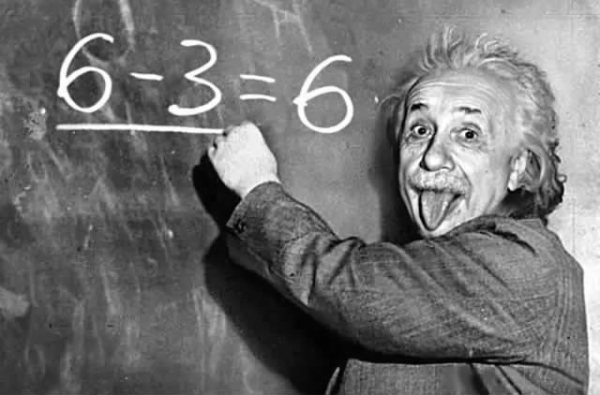
\includegraphics[width=.5\linewidth]{pictures/einstein.png}};}
				\visible<4->{\node at(4,0) {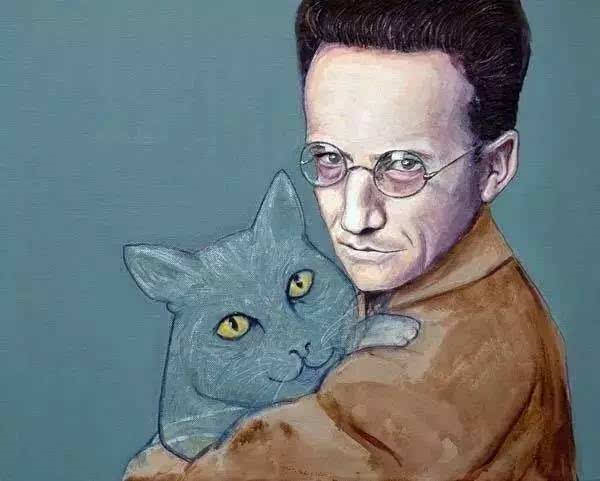
\includegraphics[width=.4\linewidth]{pictures/cat.png}};}
			\end{tikzpicture}
		\end{figure}
	\end{frame}

	\section{两种规划与学习结合的方法}
	
	\subsection{Dyna}
	
	\begin{frame}{Dyna}{主要思想和结构}
		\begin{figure}
			\centering
			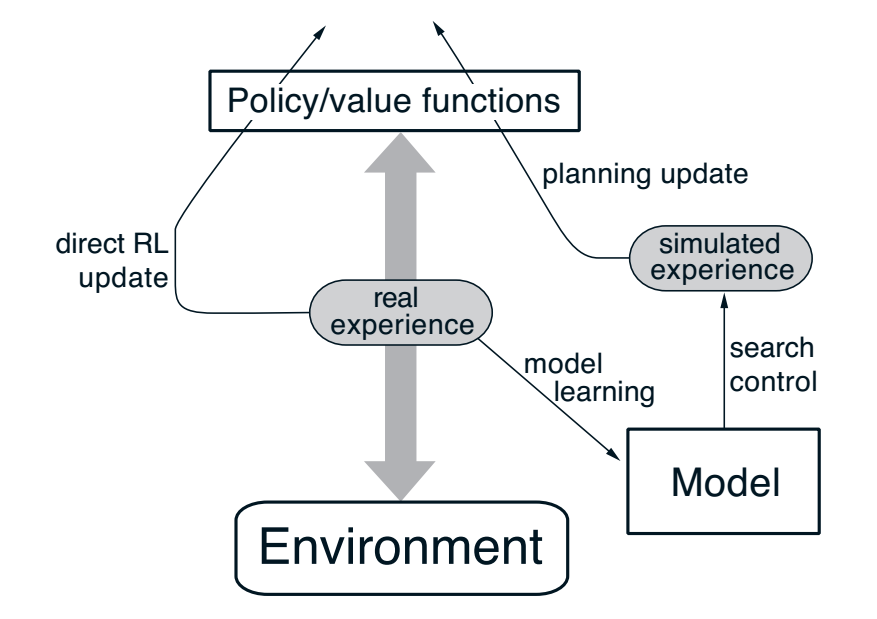
\includegraphics[width=0.6\linewidth]{pictures/dyna-arch.png}
			\caption{Dyna agent的一般结构}
			\label{fig:dyna-arch}
		\end{figure}
		
		\begin{itemize}
			\item<2-> Dyna\cite{Sutton1990:Dyna}包括了图\ref{fig:relation-in-RL}中的所有过程,即\alert{规划}、\alert{执行}、\alert{模型学习}和\alert{值函数学习}
			\item<3-> 规划时使用一个确定的模型(即$P(s,a,s') \rightarrow \{0,1\}$),该模型在;执行过程中不断更新;
		\end{itemize}
	\end{frame}

	\begin{frame}{Dyna}{Dyna-Q}
		\begin{algorithm}[H]
			对任意的$s \in S$,$a \in A(s)$,初始化$Q(s,a)$和$Model(s,a)$\;
			\Repeat{stop}{
				对当前状态$s$,根据$Q$表选择$a \in A(s)$并执行,得$s'$和$r$\;
				更新$Q(s,a)$\;
				\textcolor{blue}{用$s',r$更新$Model(s,a)$\;}
				\alert{
				\Repeat(\tcp*[f]{在$Model$上规划并更新$Q$}){$N$次循环}{
					$s$为任意观察到的状态,$a$为$s$上进行过的任意操作\;
					$s',r \gets Model(s,a)$\;
					$Q(s,a) \gets Q(s,a) + \alpha [r + \gamma\max_{a'}Q(s',a') - Q(s,a)]$\;
				}}
			}
			\caption{Dyna-Q算法}\label{alg:dyna-q}
		\end{algorithm}
	\end{frame}

	\begin{frame}{Dyna}{实验}
		\begin{figure}
			\centering
			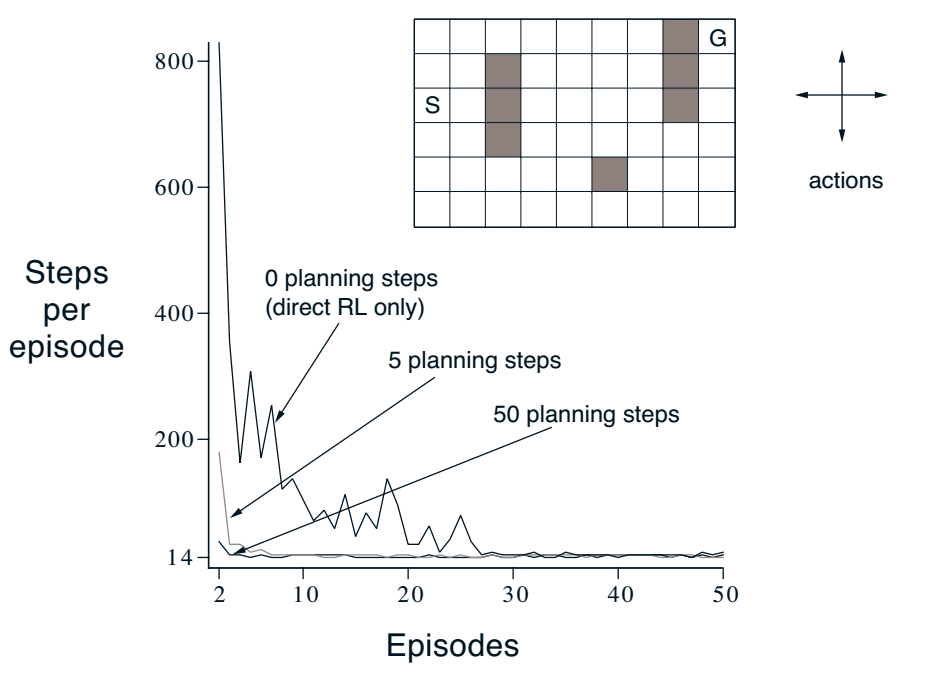
\includegraphics[width=0.7\linewidth]{pictures/dyna-exp}
			\caption[Dnya-Q 迷宫]{Dyna-Q在一个迷宫问题上的实验,agent需要从S走到G,$r\rightarrow \{0,1\}$。对于所有的$N$,第一次探索是一样的,都是大约1700步;之后,Dyna-Q和Q-Learning的差别开始显现}
			\label{fig:dyna-exp}
		\end{figure}
	\end{frame}

	\begin{frame}{Dyna}{错误的模型-原因}
		模型出错的原因:
		\begin{itemize}
			\item 先验知识存在错误
			\item 随机环境难以用模型描述或估计
			\item 环境出现变化
		\end{itemize}
		
		处理方法:学习过程中不断使用从环境中获得的数据对模型进行更新和纠正
	\end{frame}
	
	\begin{frame}{Dyna}{错误的模型-实验}
		\begin{figure}
			\centering
			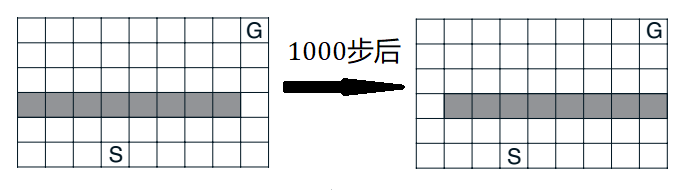
\includegraphics[width=0.5\linewidth]{pictures/blocking-maze}
			\caption{1000步之后,迷宫出现变化,左侧墙壁打开,右侧通路封闭}
			\label{fig:blocking-maze}
		\end{figure}
		
		\visible<2->{
			\begin{figure}
				\centering
				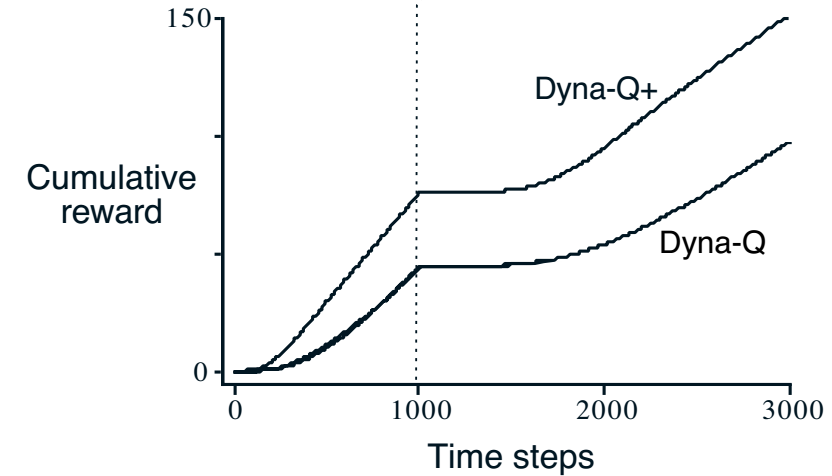
\includegraphics[width=0.5\linewidth]{pictures/blocking-maze-result}
				\caption{由于Dyna算法包括了对模型的更新,agent在一段时间后完成了对环境的重新建模并找到了正确的路径。图中Q+是加强了探索能力的Q-Learning,用$r+\kappa \sqrt{n}$为奖励函数,$n$为$s$状态下$a$连续未被选中的次数}
				\label{fig:blocking-maze-result}
			\end{figure}
		}
	\end{frame}
	
	\subsection{DARLING}
	
	\begin{frame}{DARLING}{方法介绍}
		DARLING方法\cite{Leonetti2016:AutoPlan-RL}的求解步骤:
		\begin{enumerate}
			\item<2-> 根据预设的模型,用规划求解器(例如ASP推理机)求解某个度量值(例如规划的步骤数量)在阈值内的规划方案;
			\item<3-> 筛选合并求得的规划方案,删除包含冗余步骤的方案,融合后得到部分策略,即在各个状态下可选的行动集合;
			\item<4-> 执行和学习,在执行中仅选择部分策略中的行为,学习它们的累积奖励的期望并优化策略。
		\end{enumerate}
	
	\end{frame}

	\begin{frame}{DARLING}{建模,规划,筛选,合并}
		\begin{description}
			\item<2->[建模(Modeling)] 对环境$D=\langle S, A, P, r,\gamma \rangle$进行建模,建立从环境状态到模型状态的函数$o:S \rightarrow S_m$,得$D_m = \langle S_m, A, P_m \rangle$,其中
			\item<3->[规划(Planning)] 利用规划工具,以一定的冗余度计算可行的方案。规划是在一个假设的模型上执行的,因此不能保证所得的方案是最优甚至可行的;
			\item<4->[筛选(Filtering)] 如果规划方案中存在重复出现的状态和动作(例如存在环),则认为方案是冗余的,可以被更短的方案代替;
			\item<5->[合并(Merging)] 合并筛选过的方案,得到可达状态和这些状态下可选择的动作的集合,即一个简化的模型$D_r$;
		\end{description}
		
		\vspace{10pt}
		\visible<5->{
			从Planning到Merging的过程其实是将假设中的模型$D_m$做了进一步的化简和压缩。
		}
	\end{frame}

	\begin{frame}{DARLING}{Planning \& Filtering and Merging-例}
		\begin{figure}
			\centering
			\subfigure[迷宫问题,要求机器人从S走到G,图中红色横线为一扇可能开启或关闭的门。Planning步骤求长度小于最短方案的1.5倍的方案]{
			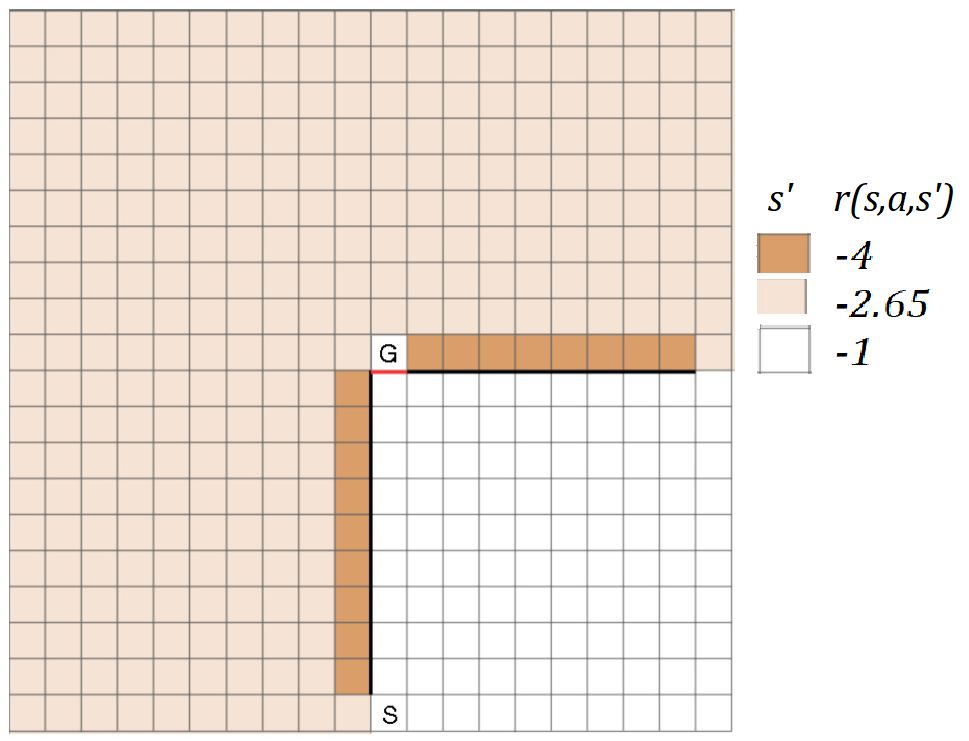
\includegraphics[width=0.475\linewidth]{pictures/grid-world.png}
			}
			\subfigure[部分策略,由筛选后的non-redudant方案融合而成]{
			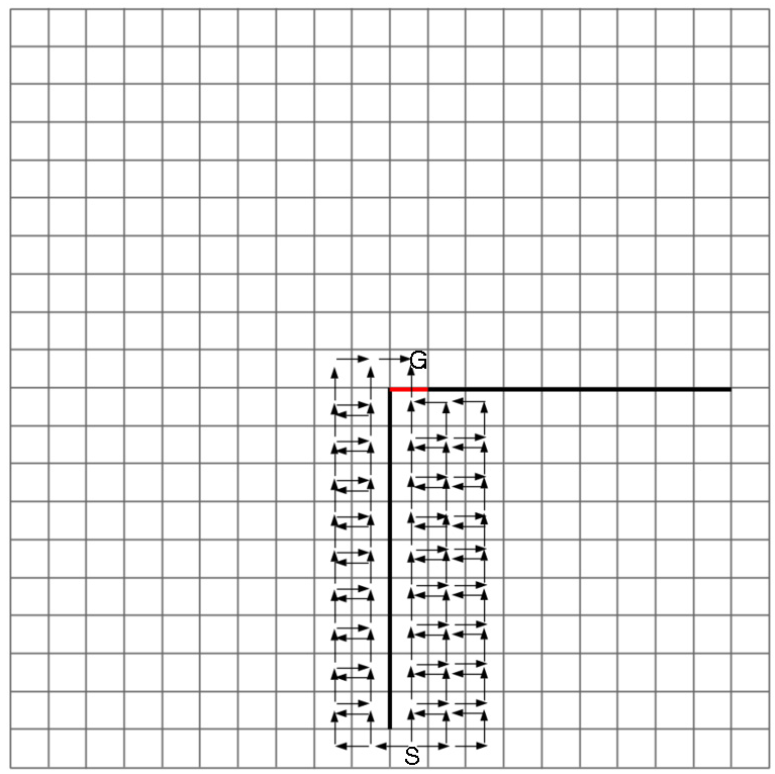
\includegraphics[width=.35\linewidth]{pictures/partial-policy.png}
			}
			\label{fig:grid-world}
		\end{figure}
	
	\end{frame}

	\begin{frame}{DARLING}{Execution and learning}
		\begin{itemize}
		\item 实际的转移函数和模型中设想的转移函数并不一致。这会导致agent在执行和学习的过程中进入了模型中没有的状态。此时应该以新出现的状态为初始状态,重新进行规划,并将所得的部分策略添加到已有的部分策略中;
		
		\item 在所得模型上的RL与其他的强化学习并无太大差别,任意的强化学习方法都可以实现。
		\end{itemize}
	\end{frame}

	\begin{frame}{DARLING}{实验}
		\begin{itemize}
			\item<2-> 实验采用的环境如图\ref{fig:grid-world}所示。仅在agent到达门口时才获知门是否打开(Partial Observed MDP,POMDP),在周期$e$时门打开的概率为
				\[p(e)=
					\begin{cases}
						1 - \frac{e}{E-1} & 0 \leq e < E \\
						0 & \text{other wise}
					\end{cases}
				\]
			\item<3-> 实验中用到了以下几种agent:
			\begin{description}
				\item[P agent]<4-> 仅在$D_m$上进行规划;
				\item[RL agent]<5-> 仅在$D$上进行强化学习;
				\item[PRL agent]<6-> 采用DARLING方法,在$D_m$上计算部分策略,并将强化学习的探索限制在$D_r$上;
				\item[Pmem-n agent]<7-> 采用DARLING方法,有前$n$个周期内观察门是否打开的记忆,并以此估计当前门是否打开;
			\end{description}
		\end{itemize}
	\end{frame}

	\begin{frame}{DARLING}{实验结果}
		\begin{figure}
			\centering
			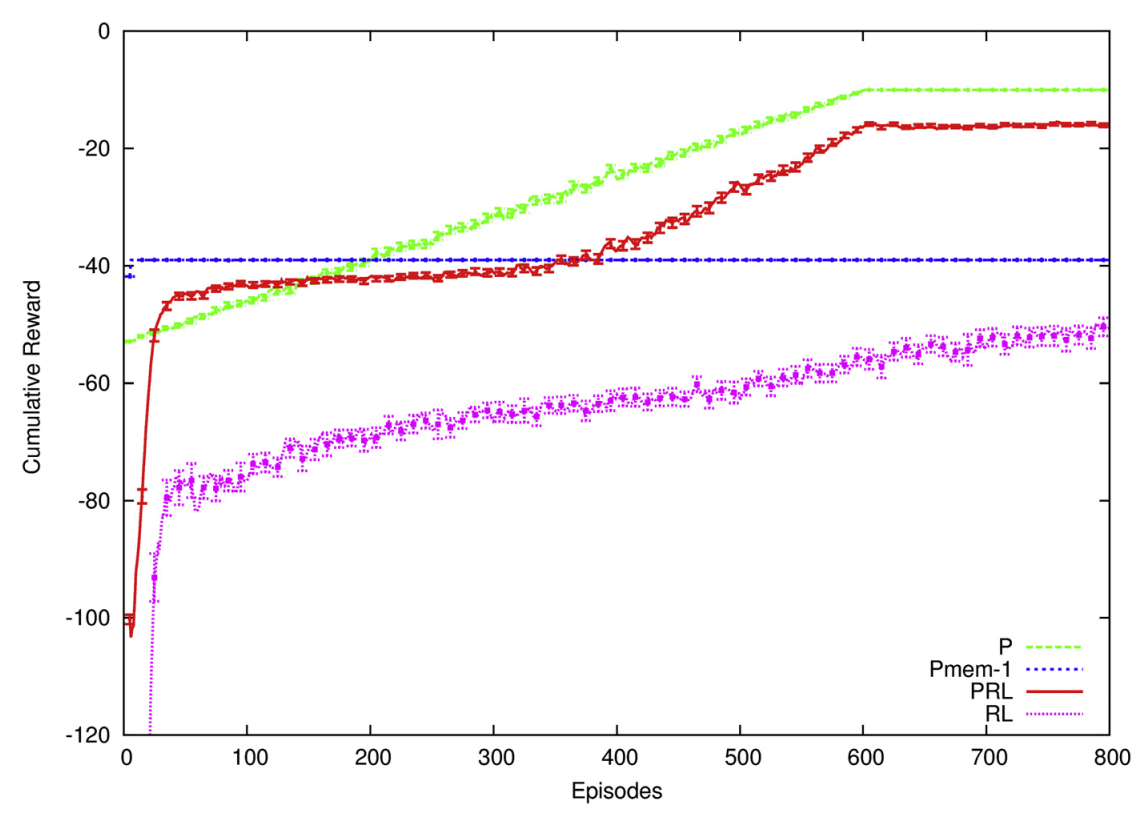
\includegraphics[width=0.6\linewidth]{pictures/darling-expr}
			\caption{实验结果}
			\label{fig:darling-expr}
		\end{figure}
		\visible<2->{
			\only<2>{P agent的累积奖励变化与$p(e)$的概率保持一致。但由于实际应用中,$D_m$和$D$差距较大,因此直接使用规划方法不可能取得如此良好的结果。}
			\only<3>{RL agent很快学到了最优策略,但环境变化后没有能发现更优的策略。}
			\only<4>{PRL agent学到了最优策略,并在环境变化后选择了更优的策略。}
			\only<5>{Pmem-1 agent被起初的观察限制,没有发现环境的变化,因此没有发现更优的策略。实际上,无论$n$的取值如何,agent在不稳定的环境中都没有获得最优策略。}
		}
	\end{frame}

	\part{事后经验回放}\label{part:her}
	
	\section{相关背景}
	
	\begin{frame}{相关背景}{简介}
		\begin{itemize}
			\item<2-> 强化学习(RL)与神经网络的结合被广泛应用于序列决策问题中;
			
			\item<3-> 一个必须要面对的问题(尤其对于机器人设计来说):通常需要设计一个回报函数(reward function),它不仅要体现目标任务,而且还要能够指导agent优化决策策略(policy optimization);
			
			\item<4-> 由此带来的问题是:这不仅需要RL专业知识,还需要领域特定的知识(domain-specific knowledge);
			
		\end{itemize}
		
		\visible<5>{Problem:能否设计一个算法,能够从unshaped reward signals(e.g. 一个0-1 reward表明任务是否成功完成)中学习?}
	\end{frame}

	\begin{frame}{背景介绍}{简介}
		\begin{figure}
			\centering
			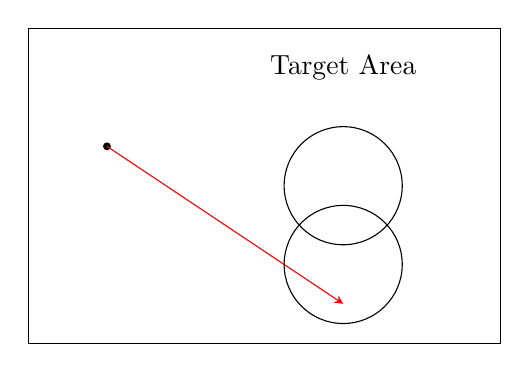
\begin{tikzpicture}
				\draw (0,0) rectangle (6cm, 4cm);
				\draw [draw=white] (4,3.5) node {Target Area};
				\draw (4,2) circle [radius=.75cm];
				\fill (1,2.5) circle [radius=.05cm,fill=black];
				\draw [->,>=stealth,draw=red] (1,2.5) -- (4,0.5);
				
				\visible<2->{\draw(4,1) circle [radius=.75cm];}
			\end{tikzpicture}
			\caption{人类拥有的一种能力是从未达到预期的结果那里获得与希望获得的结果几乎一样的知识。}\label{fig:idea-of-her}
		\end{figure}
	\end{frame}

	\begin{frame}{相关背景}{Deep Q-Networks(DQN)}
		\begin{figure}
			\centering
			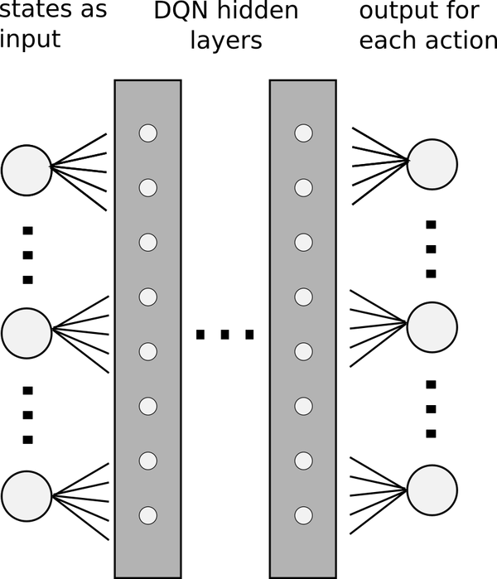
\includegraphics[width=0.4\linewidth]{pictures/DQN}
			\caption{使用神经网络来近似Q函数。该网络将一个状态s作为输入,并为每个动作a输出Q函数的估计值。}
			\label{fig:dqn}
		\end{figure}
	\end{frame}

	\begin{frame}{相关背景}{经验回放(Experience Replay)}
		\begin{itemize}
			\item 对于不可枚举状态的环境(如连续的状态空间),一般采用值函数逼近(Value Function Approxiamation)来拟合和泛化Q函数。
			
			\item 经验回放(Experience replay)是从一个memory pool中随机选取expeirence更新网络。
			
			\item DQN是基于监督学习的框架,而loss function基于RL,因此会有这样的问题:监督学习需要假设样本是独立同分布,而RL中的强序列关联性不符合这个假设。如果没有experience replay,可能会出现不收敛的情况;
			
			\item 采用Experience Replay,会缓和样本的关联性。其优点包括:
				\begin{enumerate}
					\item 算法收敛;
					\item 提高泛化能力;
				\end{enumerate}
			
		\end{itemize}
	\end{frame}

	\begin{frame}{相关背景}{Deep Deterministic Policy Gradients (DDPG)}
		\begin{itemize}
			\item<2-> DQN是一个面向离散控制的算法,即输出的动作是离散的;
			
			\item<3-> 深度确定性策略梯度(Deep Deterministic Policy Gradient, DDPG)算法是利用 DQN 扩展 Q 学习算法的思路对确定性策略梯度(Deterministic Policy Gradient, DPG)方法进行改造,提出的一种基于行动者-评论家(Actor-Critic,AC)框架的算法,该算法可用于解决连续动作空间上的 DRL 问题。
			
			\item<4-> 随机性策略和确定性策略:
				\begin{description}
					\item[随机性策略]<5-> 策略输出的是动作的概率,比如连续动作控制,使用的是一个正态分布对动作进行采样选择,即每个动作都有概率被选到;
						\begin{description}
							\item[优点] 将探索和改进集成到一个策略中;
							\item[缺点] 需要大量训练数据;
						\end{description}
					
					\item [确定性策略]<6-> 策略输出即是动作
						\begin{description}
							\item[优点] 需要采样的数据少,算法效率高;
							\item[缺点] 无法探索环境;
						\end{description}
				\end{description}
			
		\end{itemize}
	\end{frame}
	
	\section{事后经验回放(HER)}
	
	\begin{frame}{HER}{启发案例-I}
		\begin{example}
			\begin{columns}
				\begin{column}{0.5\textwidth}
					\begin{itemize}
						\item 环境描述:
							\begin{description}
								\item[状态空间] $S = \{0,1\}^n$
								\item[动作空间] $\{0, 1, \dots, n-1 \}$
								\item[奖励函数] $r(s,a) = -\sgn(s \neq g)$
							\end{description}	
					\end{itemize}
					
				\end{column}
				\begin{column}{0.5\textwidth}
					\begin{figure}
						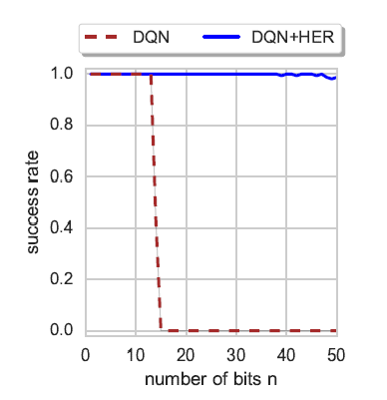
\includegraphics[width=.7\linewidth]{pictures/bit-flip.png}
						\caption{Bit Flipping实验结果}\label{fig:bi-flip}
					\end{figure}
				\end{column}
			\end{columns}
		
			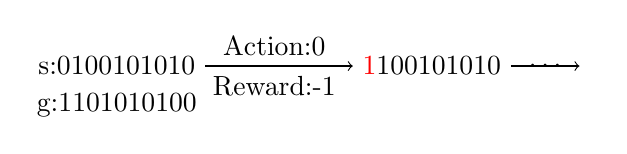
\begin{tikzpicture}
				\node [draw opacity=0] (s) at (0,.5) {s:0100101010};
				\node [draw opacity=0] (g) at(0,0) {g:1101010100};
				\visible<3-> {
					\node [draw opacity=0,right of=s] (s1) at (3,.5) {\textcolor{red}{1}100101010};
					\path [->] (s) edge (s1);
				}
				\visible<2-> {
					\node [draw opacity=0] (a) at (2,.75) {Action:0};
				}
				\visible<4-> {
					\node [draw opacity=0] (r) at (2,.25) {Reward:-1};
				}
				\visible<5-> {
					\node [draw opacity=0] (v) at (6,.5) {};
					\path [->] (s1) edge node (dot) {$\cdots$} (v);
				}
			\end{tikzpicture}
		\end{example}
	\end{frame}

	\begin{frame}{HER}{启发案例-II}
		\begin{itemize}
			\item<2-> 在这样的环境下,尤其是比特位数$n$>40时,经典的强化学习算法如DQN很难学习到从起始状态到终点状态的路径;因为它探索到的reward值基本都是-1;
			
			\item<3-> 在这样的环境中,一个比较好的解决方法是用一个shaped reward function,以此来给予agent更多到达终点的信息;如: $r_g(s,a) = -||s - g||^2 $;
			
			\item<4-> 在更为复杂的环境中,设置一个有效的合适的回报函数有时会比较困难;因此本文目的是设计一个更为普遍的通用于多种环境中的方法,而不要有针对环境的特定领域知识。
			
		\end{itemize}
	\end{frame}

	\begin{frame}{HER}{多目标强化学习(Multi-goal RL )}
		\begin{itemize}
			\item 训练agent能够学会到达多个目标点;
				\[f_g \left( (x,y) \right) =  \sgn(s=g) \]
			
			\item 使用Universal Value Function Approximators,在训练policy和value function的过程中,将state $s$和目标$g$作为输入;
		\end{itemize}
		
	\end{frame}

	\begin{frame}{HER}{算法描述}
		\begin{figure}
			\centering
			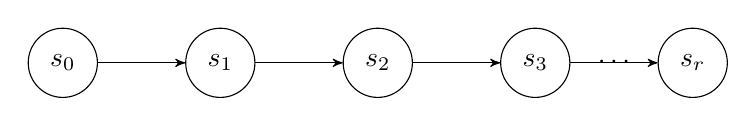
\begin{tikzpicture}[->,>=stealth',node distance=2cm]
				\node [state] (s0) {$s_0$};
				\node [state,right of=s0] (s1) {$s_1$};
				\node [state,right of=s1] (s2) {$s_2$};
				\node [state,right of=s2] (s3) {$s_3$};
				\node [state,right of=s3] (sr) {$s_r$};
				\path (s0) edge (s1)
						  (s1) edge (s2)
						  (s2) edge (s3)
						  (s3) edge node {$\cdots$} (sr);
			\end{tikzpicture}
		\end{figure}
	
		\begin{algorithm}[H]
			A episode: $s_0,s_1,s_2,…, s_T$\;
			
			\ForEach{Time-stem $t$}{
				使用现有的策略A,从中选取一个action$a_t$,即$a_t \gets \pi_b (s_t ||g)$\;
				计算reward值:$r_t=r(s_t,a_t,g)$\;
				Experience Replay: 将状态转移$s_t \rightarrow s_(t+1)$以$(s_t ||g,a_t,r_t,s_(t+1)||g)$形式保存到replay buffer中\;
			}
			利用replay buffer 进行更新已有策略A\;
			\caption{事后经验回放算法}\label{alg:her}
		\end{algorithm}
	\end{frame}
	
	\section{实验}
	
	\begin{frame}{实验}{环境}
		\begin{itemize}
			\item 采用在现有的硬件机器人的基础上的控制环境
			\item 可用一个物理引擎模拟机器人的控制和反馈
				\begin{figure}
					\centering
					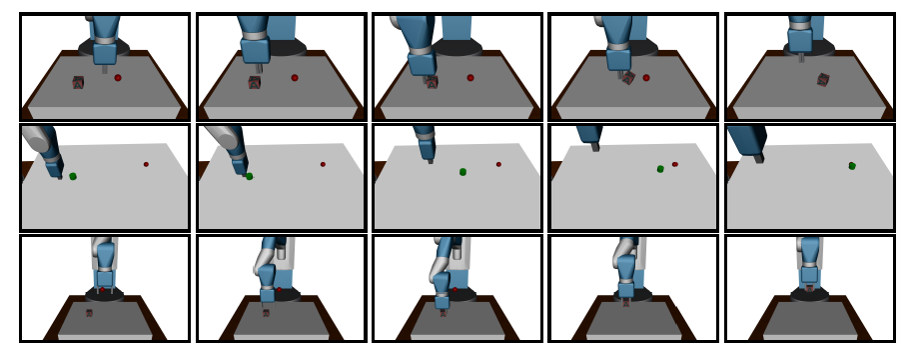
\includegraphics[width=0.7\linewidth]{pictures/her-robot}
					\caption{三种不同的任务:pushing(第一行),sliding(第二行),pick and place(第三行)}
					\label{fig:her-robot}
				\end{figure}
				
		\end{itemize}
	\end{frame}

	\begin{frame}{实验}{三种任务}
		\begin{description}
			\item[Pushing] A box is placed on a table in front of the robot and the task is to move it to the target location on the table. The robot fingers are locked to prevent grasping. The learned behavior is a mixture of pushing and rolling.
			
			\item[Sliding] A puck is placed on a long slippery table and the target position is outside of the robot’s reach so that it has to hit the puck with such a force that it slides and then stops in the appropriate place due to friction.
			
			\item[Pick-and-place] The target position is in the air and the fingers are not locked. 
			
		\end{description}
	\end{frame}

	\begin{frame}{实验}{模型}
		\begin{description}
			\item[States] The state of the system is represented in the MuJoCo physics engine and consists of angles and velocities of all robot joints as well as positions, rotations and velocities (linear and angular) of all objects.
			
			\item[Goals] Goals describe the desired position of the object (a box or a puck depending on the task) with some fixed tolerance of $\epsilon$, i.e. , $f_g(s) = \sgn(g-s_{object} \leq \epsilon)$. 
			
			\item[Rewards] Use binary and sparse rewards $\{−1,0\}$;
			
			\item[State-goal distributions] For all tasks the initial position of the gripper is fixed, while the initial position of the object and the target are randomized;
			
		\end{description}
	\end{frame}
	
	\begin{frame}{实验}{多目标学习结果}
		\begin{figure}
			\centering
			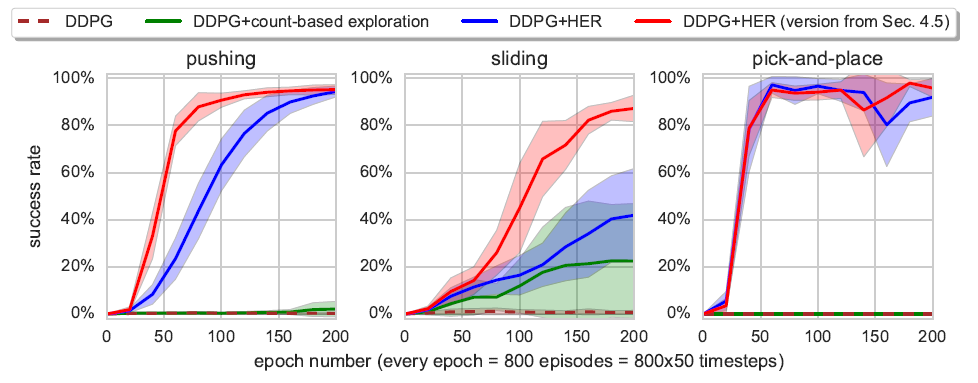
\includegraphics[width=0.7\linewidth]{pictures/multi-goal-expr}
			\caption{多目标学习曲线}
			\label{fig:multi-goal-expr}
		\end{figure}
		
	\end{frame}

	\begin{frame}{实验}{单目标学习结果}
		\begin{figure}
			\centering
			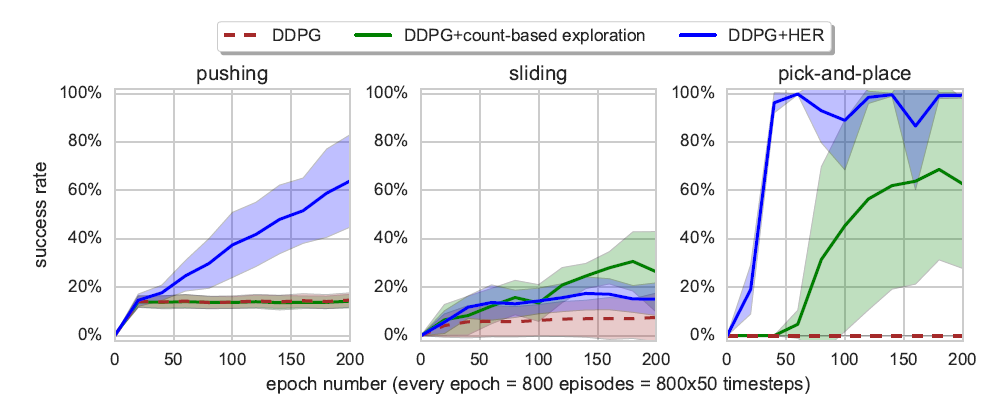
\includegraphics[width=0.7\linewidth]{pictures/single-goal-expr}
			\caption{单目标学习曲线}
			\label{fig:single-goal-expr}
		\end{figure}
		
	\end{frame}

	\begin{frame}{实验}{奖励函数变更结果}
		\begin{figure}
			\centering
			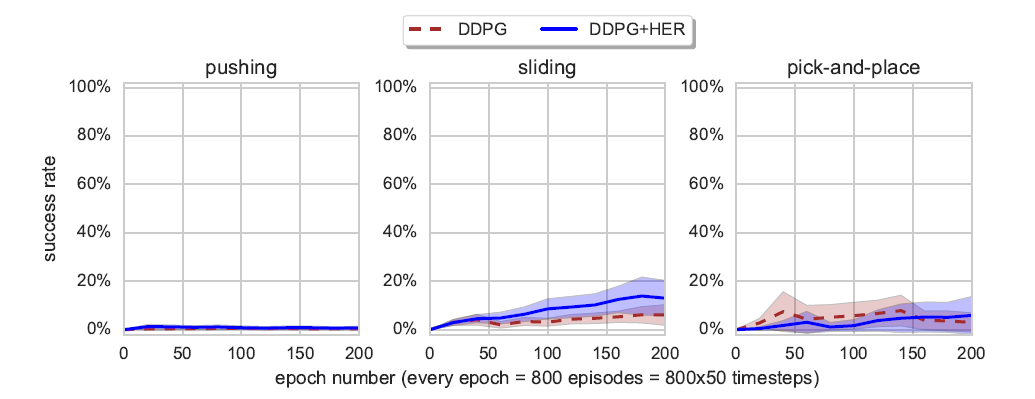
\includegraphics[width=0.7\linewidth]{pictures/reward-shape-expr}
			\caption{变更奖励函数后的学习曲线,其中$r(s,a,g) = -|g-s'_{object}|^2$}
			\label{fig:reward-shape-expr}
		\end{figure}
		
	\end{frame}

	\section{结论}
	
	\begin{frame}{结论}
		\begin{enumerate}
			\item 提出了HER算法,能够将强化学习方法应用到稀疏回报值的问题中;
			\item HER算法具有很强的通用性,能够结合任意的off-policy RL算法,在实验中结合的是DQN和DDPG方法;
			\item 在实验中,将HER算法应用到让机器臂完成不同的移动物品的任务上,展示了突出的效果。
		\end{enumerate}
	\end{frame}
		
	\part{强化学习在游戏中的应用}\label{part:rl-in-fps}
	
	\section{Atari游戏与DQN}
	
	\section{FPS游戏与DRQN}
	
	\section*{参考文献}
	
	\begin{frame}{参考文献}
		\bibliographystyle{apalike}
		\bibliography{reference}
	\end{frame}
	
	{\background%末页致谢
		\begin{frame}[plain,noframenumbering]
			\finalpage{{\huge 感谢观看!\\ \small Q \& A}}
		\end{frame}
	}
	
\end{document}